%% abtex2-modelo-relatorio-tecnico.tex, v<VERSION> laurocesar
%% Copyright 2012-2015 by abnTeX2 group at http://abntex2.googlecode.com/ 
%%
%% This work may be distributed and/or modified under the
%% conditions of the LaTeX Project Public License, either version 1.3
%% of this license or (at your option) any later version.
%% The latest version of this license is in
%%   http://www.latex-project.org/lppl.txt
%% and version 1.3 or later is part of all distributions of LaTeX
%% version 2005/12/01 or later.
%%
%% This work has the LPPL maintenance status `maintained'.
%% 
%% The Current Maintainer of this work is the abnTeX2 team, led
%% by Lauro César Araujo. Further information are available on 
%% http://abntex2.googlecode.com/
%%
%% This work consists of the files abntex2-modelo-relatorio-tecnico.tex,
%% abntex2-modelo-include-comandos and abntex2-modelo-references.bib
%%

% ------------------------------------------------------------------------
% ------------------------------------------------------------------------
% abnTeX2: Modelo de Relatório Técnico/Acadêmico em conformidade com 
% ABNT NBR 10719:2011 Informação e documentação - Relatório técnico e/ou
% científico - Apresentação
% ------------------------------------------------------------------------ 
% ------------------------------------------------------------------------

\documentclass[
	% -- opções da classe memoir --
	12pt,				% tamanho da fonte
	openright,			% capítulos começam em pág ímpar (insere página vazia caso preciso)
	oneside,			% para impressão em verso e anverso. Oposto a oneside
	a4paper,			% tamanho do papel. 
	% -- opções da classe abntex2 --
	%chapter=TITLE,		% títulos de capítulos convertidos em letras maiúsculas
	%section=TITLE,		% títulos de seções convertidos em letras maiúsculas
	%subsection=TITLE,	% títulos de subseções convertidos em letras maiúsculas
	%subsubsection=TITLE,% títulos de subsubseções convertidos em letras maiúsculas
	% -- opções do pacote babel --
	english,			% idioma adicional para hifenização
	french,				% idioma adicional para hifenização
	spanish,			% idioma adicional para hifenização
	brazil,				% o último idioma é o principal do documento
	]{abntex2}

% ---
% PACOTES
\include{auxiliares/pacotes}
% --- 
% CONFIGURAÇÕES DE PACOTES
% --- 

% ---
% Configurações do pacote backref
% Usado sem a opção hyperpageref de backref
\renewcommand{\backrefpagesname}{Citado na(s) página(s):~}
% Texto padrão antes do número das páginas
\renewcommand{\backref}{}
% Define os textos da citação
\renewcommand*{\backrefalt}[4]{
	\ifcase #1 %
		Nenhuma citação no texto.%
	\or
		Citado na página #2.%
	\else
		Citado #1 vezes nas páginas #2.%
	\fi}%
% ---

% Altera o nome padrão do rótulo usado no comando \autoref{}
\renewcommand{\lstlistingname}{Código}

% Altera o rótulo a ser usando no elemento pré-textual "Lista de código"
\renewcommand{\lstlistlistingname}{Lista de códigos}

% Configura a ``Lista de Códigos'' conforme as regras da ABNT (para abnTeX2)
\begingroup\makeatletter
\let\newcounter\@gobble\let\setcounter\@gobbletwo
  \globaldefs\@ne \let\c@loldepth\@ne
  \newlistof{listings}{lol}{\lstlistlistingname}
  \newlistentry{lstlisting}{lol}{0}
\endgroup

\renewcommand{\cftlstlistingaftersnum}{\hfill--\hfill}

\let\oldlstlistoflistings\lstlistoflistings
\renewcommand{\lstlistoflistings}{%
   \begingroup%
   \let\oldnumberline\numberline%
   \renewcommand{\numberline}{\lstlistingname\space\oldnumberline}%
   \oldlstlistoflistings%
   \endgroup}


\definecolor{mygreen}{rgb}{0,0.6,0}
\definecolor{mygray}{rgb}{0.5,0.5,0.5}
\definecolor{mymauve}{rgb}{0.58,0,0.82}

\lstset{ %
  backgroundcolor=\color{white},   % choose the background color; you must add \usepackage{color} or \usepackage{xcolor}
  basicstyle=\footnotesize,        % the size of the fonts that are used for the code
  breakatwhitespace=false,         % sets if automatic breaks should only happen at whitespace
  breaklines=true,                 % sets automatic line breaking
  captionpos=b,                    % sets the caption-position to bottom
  commentstyle=\color{mygreen},    % comment style
  deletekeywords={...},            % if you want to delete keywords from the given language
  escapeinside={\%*}{*)},          % if you want to add LaTeX within your code
  extendedchars=true,              % lets you use non-ASCII characters; for 8-bits encodings only, does not work with UTF-8
  frame=single,                    % adds a frame around the code
  keepspaces=true,                 % keeps spaces in text, useful for keeping indentation of code (possibly needs columns=flexible)
  keywordstyle=\color{blue},       % keyword style
  language=Octave,                 % the language of the code
  otherkeywords={*,...},            % if you want to add more keywords to the set
  numbers=left,                    % where to put the line-numbers; possible values are (none, left, right)
  numbersep=5pt,                   % how far the line-numbers are from the code
  numberstyle=\tiny\color{mygray}, % the style that is used for the line-numbers
  rulecolor=\color{black},         % if not set, the frame-color may be changed on line-breaks within not-black text (e.g. comments (green here))
  showspaces=false,                % show spaces everywhere adding particular underscores; it overrides 'showstringspaces'
  showstringspaces=false,          % underline spaces within strings only
  showtabs=false,                  % show tabs within strings adding particular underscores
  stepnumber=2,                    % the step between two line-numbers. If it's 1, each line will be numbered
  stringstyle=\color{mymauve},     % string literal style
  tabsize=2,                       % sets default tabsize to 2 spaces
  title=\lstname                   % show the filename of files included with \lstinputlisting; also try caption instead of title
}   
   
   
   
%%%%%% Configurações do pacote Tikz para diagramas
\tikzstyle{block} = [rectangle, draw, fill=blue!20, 
    text width=5em, text centered, rounded corners, minimum height=4em]
\tikzstyle{line} = [draw, -latex']

%%%%% Configuração do PGFPlots
\pgfplotsset{compat=1.11}
\usetikzlibrary{patterns}
%\newcommand{\imprimeNumeroContrato}{}
%\newcommand{\imprimeValorProduto}{}
%\newcommand{\imprimeValorContrato}{}
%\newcommand{\imprimeDataEntrega}{}
%\newcommand{\imprimeLabelSupervisor}{}
%\newcommand{\imprimeSupervisor}{}
%\newcommand{\numeroContrato}[1]{\renewcommand{\imprimeNumeroContrato}{#1}}
%\newcommand{\valorProduto}[1]{\renewcommand{\imprimeValorProduto}{#1}}
%\newcommand{\valorContrato}[1]{\renewcommand{\imprimeValorContrato}{#1}}
%\newcommand{\dataEntrega}[1]{\renewcommand{\imprimeDataEntrega}{#1}}
%\newcommand{\supervisor}[2][Nome do supervisor]{%
%\renewcommand{\imprimeLabelSupervisor}{#1}%
%\renewcommand{\imprimeSupervisor}{#2}%
%}

%Needs xparse package - Dual Entry for glossary (glossary + acronym)
\DeclareDocumentCommand{\newdualentry}{ O{} O{} m m m m } {
  \newglossaryentry{gls-#3}{name={#5},text={#5\glsadd{#3}},
    description={#6},sort={#3}
  }
  \newacronym[see={[Glossário: ]{gls-#3}},#2]{#3}{#4}{#5\glsadd{gls-#3}}
}
% ---
% Informações de dados para CAPA e FOLHA DE ROSTO
% ---
\titulo{Produto 2 - Relatório contendo proposta de solução para gerar relatório agregado que consolide e organize as contribuições recebidas através ferramentas e aplicações de consulta pública}
\autor{Diego Rabatone Oliveira}
\local{Brasil}
\data{Abril/2015, v1}
\newcommand{\numeroContrato}{2015/000042-00}
\newcommand{\valorProduto}{R\$6.200,00 (seis mil e duzentos reais)}
\newcommand{\valorContrato}{R\$40.000,00 (quarenta mil reais}
\newcommand{\dataEntrega}{08/03/2015}
\newcommand{\labelSupervisor}{Supervisora}
\newcommand{\supervisor}{Sabrina Durigon Marques}
\instituicao{%
  Secretaria de Assuntos Legislativos do 
  \par
  Ministério da Justiça (SAL/MJ)}
\orientador[Supervisora:]{Sabrina Durigon Marques}

\tipotrabalho{Relatório técnico}
% O preambulo deve conter o tipo do trabalho, o objetivo, 
% o nome da instituição e a área de concentração 
\preambulo{Relatório referente ao Projeto BRA/07/004 – Democratização de Informações no Processo de Elaboração Normativa}
% ---

% ---
% Configurações de aparência do PDF final

% alterando o aspecto da cor azul
\definecolor{blue}{RGB}{41,5,195}

% informações do PDF
\makeatletter
\hypersetup{
     	%pagebackref=true,
		pdftitle={\@title}, 
		pdfauthor={\@author},
    	pdfsubject={\imprimirpreambulo},
	    pdfcreator={LaTeX with abnTeX2},
		pdfkeywords={marco civil da internet}{proteção de dados pessoais}{métodos ágeis}, 
		colorlinks=true,       		% false: boxed links; true: colored links
    	linkcolor=blue,          	% color of internal links
    	citecolor=blue,        		% color of links to bibliography
    	filecolor=magenta,      		% color of file links
		urlcolor=blue,
		bookmarksdepth=4
}
\makeatother
% --- 
% ---
% compila o indice
\makeindex
\makeglossaries

%\begin{siglas}
%  \item[ABNT] Associação Brasileira de Normas Técnicas
%  \item[abnTeX] ABsurdas Normas para TeX
%\end{siglas}

%\newacronym%
%[description={}]%
%{}{}{}%

%\hyphenation{Django}%
%\newglossaryentry{django}{%
%    name=Django,%
%    description={\'{e} um framework para desenvolvimento r\'{a}pido para web, escrito em %Python, que utiliza o padr\~{a}o MVT}%
%}%
%\newdualentry{mvc}{MVC}{\textit{Model View Controller}}{\textit{Design Pattern} muito conhecida e introduzida por \textit{Erich Gamma} em 1995}
%\newacronym{html}{HTML}{HyperText Markup Language}

\newacronym{sal}{SAL/MJ}{Secretaria de Assuntos Legislativos do Ministério da Justiça}
\newacronym{pnud}{PNUD}{Programa das Nações Unidas para o Desenvolvimento}
\newacronym{anatel}{Anatel}{Agência Nacional de Telecomunicações}
\newacronym{pnad}{PNAD}{Pesquisa Nacional por Amostra de Domicílio}
\newacronym{ibge}{IBGE}{Instituto Brasileiro de Geografia e Estatística}
\newcommand{\mc}{Marco Civil da Internet}
\newcommand{\pdp}{Proteção de Dados Pessoais}

\newglossaryentry{issue}{
	name=\textit{issue},
	description={Uma tarefa a ser realizada. No escopo deste projeto deve-se buscar a formulação de tarefas minimalistas}
}
\newglossaryentry{milestone}{
	name=\textit{milestone},
	description={Conjunto de tarefas (\textit{issues}) com prazo de finalização, neste projeto está sendo utilizado como organizador dos \textit{Sprints}}
}
\newglossaryentry{sprint}{
	name=\textit{sprint},
	description={é a unidade básica de desenvolvimento, no caso deste projeto é o trabalho (a ser) realizado durante uma semana}
}
\newglossaryentry{integrador}{
	name=integrador,
	description={Papel na equipe de desenvolvimento do responsável por realizar a integração do que foi desenvolvido pela equipe ao repositório principal do projeto}
}

\newglossaryentry{label}{
	name=\textit{label},
	description={``Etiqueta'' que pode ser adicionada a uma \textit{issue} para melhor caracterização e organização das \textit{issues}}
}

\newglossaryentry{branch}{
	name=\textit{branch},
	plural=\textit{branches},
	description={é uma ramificação na árvore de desenvolvimento do projeto no sistema de versionamento git. Para mais informações ver: \url{http://git-scm.com/book/pt-br/v1/Ramificação-Branching-no-Git-O-que-é-um-Branch}}
}

\newglossaryentry{merge}{
	name=\textit{merge},
	description={é a ação de agregar propostas de modificação de diferentes \textit{branches} ou \textit{forks}}
}

\newglossaryentry{fork}{
	name=\textit{fork},
	description={é uma cópia do projeto que tem seu desenvolvimento acontecendo de forma independente da árvore de desenvolvimento do projeto original}
}

\newglossaryentry{hotfix}{
	name=\textit{hotfix},
	plural=\textit{HotFixes},
	description={é o desenvolvimento emergencial para a resolução de algum problema do sistema que está em produção. HotFixes possuem prioridade máxima e ocorrem fora do ciclo padrão de gestão do projeto}
}

\newglossaryentry{deploy}{
	name=\textit{deploy},
	description={ação de implementar um serviço, ou atualização de um serviço, para que o mesmo possa ser utilizado pelos usuários}
}

\newglossaryentry{synset}{
	name=\textit{synset},
	plural=\textit{synsets},
	description={é um conjunto de sinônimos cognitivos, ou seja, um conjunto de verbos que expressam um mesmo conceito}
}

\newglossaryentry{toolkit}{
	name=\textit{toolkit},
	plural=\textit{toolkits},
	description={é um conjunto de ferramentas para realizar diferentes tarefas dentro de um mesmo escopo de atividade ou trabalho}
}

%\newdualentry{pullrequest}{PR}{\textit{pull-request}}{requisição realizada com propostas de modificação no código fonte do repositório principal do projeto}

\newdualentry{seo}{SEO}{\textit{Search Engine Optimization}}{conjunto de estratégias com o objetivo de potencializar e melhorar o posicionamento de um site nas páginas de resultados naturais (orgânicos) nos sites de busca.}

%\newdualentry{pln}{PLN}{Processamento de Linguagem Natual}{é uma subárea da inteligência artificial e da linguística que estuda os problemas da geração e compreensão automática de linguas humanas naturais}

%\newdualentry{nlp}{NLP}{\textit{Natural Language Processing}}{termo em inglês para Processamento de Linguagem Natural}

\glsresetall
%\glsaddsall
\renewcommand*{\glsseeformat}[3][\seename]{\textit{#1}\glsseelist{#2}}

% ----
% Início do documento
\begin{document}
\pagestyle{estilosalmj}
\aliaspagestyle{chapter}{estilosalmj}% customizing chapter pagestyle

% Seleciona o idioma do documento (conforme pacotes do babel)
%\selectlanguage{english}
\selectlanguage{brazil}

% Retira espaço extra obsoleto entre as frases.
\frenchspacing 

% ----------------------------------------------------------
% ELEMENTOS PRÉ-TEXTUAIS

% ---
% Capa
\imprimircapa

% ---
% Folha de rosto
% (o * indica que haverá a ficha bibliográfica)
\imprimirfolhaderosto*

% ---
% Anverso da folha de rosto:

{
\ABNTEXchapterfont

\begin{fichacatalografica}
	\sffamily
	\vspace*{\fill}					% Posição vertical
	\begin{center}					% Minipage Centralizado
	\fbox{\begin{minipage}[c][8cm]{13.5cm}		% Largura
	\small
	\imprimirautor
	%Sobrenome, Nome do autor
	
	\hspace{0.5cm} \imprimirtitulo  / \imprimirautor. --
	\imprimirlocal, \imprimirdata-
	
	\hspace{0.5cm} \pageref{LastPage} p. : il. (algumas color.) ; 30 cm.\\
	
	\hspace{0.5cm} \imprimirorientadorRotulo~\imprimirorientador\\
	
	\hspace{0.5cm}
	\parbox[t]{\textwidth}{\imprimirtipotrabalho~--~\imprimirinstituicao,
	\imprimirdata.}\\
	
	\hspace{0.5cm}
		1. Pensando O Direito.
		2. Participação Social.
		I. Sabrina Durigon Marques.
		II. Secretaria de Assuntos Legislativos.
		III. Ministério da Justiça.
		IV. \imprimirtitulo
	\end{minipage}}	
	\end{center}

	\footnotesize{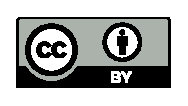
\includegraphics[scale=0.5]{./imagens/ccby.eps} Este trabalho está licenciado com uma Licença \href{http://creativecommons.org/licenses/by/4.0/}{Creative Commons - Atribuição 4.0 Internacional}.}
\end{fichacatalografica}

}

% ---
% Agradecimentos
\include{textos/agradecimentos}

% ---
% RESUMO
% resumo na língua vernácula (obrigatório)
\setlength{\absparsep}{18pt} % ajusta o espaçamento dos parágrafos do resumo
\begin{resumo}

 \noindent
 \textbf{Palavras-chaves}: Redes Sociais, relatório.
\end{resumo}
% ---


% ---
% inserir lista de símbolos
\include{textos/simbolos}

% ---
% inserindo listas (tabelas, ilustrações, etc.)
% inserir lista de ilustrações
\pdfbookmark[0]{\listfigurename}{lof}
\listoffigures
\cleardoublepage
% ---

% ---
% inserir lista de tabelas
% ---
%\pdfbookmark[0]{\listtablename}{lot}
%\listoftables*
%\cleardoublepage
% ---

%Glossário e Siglas
\printglossaries
\cleardoublepage


% ---
% inserir o sumario
% ---
\pdfbookmark[0]{\contentsname}{toc}
\tableofcontents*
\cleardoublepage
% ---


% ----------------------------------------------------------
% ELEMENTOS TEXTUAIS
% ----------------------------------------------------------
\textual
\pagestyle{estilosalmj}
\aliaspagestyle{chapter}{estilosalmj}% customizing chapter pagestyle

% ---
% Introdução
%------
%Se deseja-se o capítulo listado no índice mas que apareça aqui sem numeração.
%--
%\chapter*[Introdução]{Introdução}
%\addcontentsline{toc}{chapter}{Introdução}
%------
\chapter{Introdução}
	O Projeto Pensando o Direito é uma iniciativa da \gls{sal}, e foi criado em 2007 para promover a democratização do processo de elaboração legislativa no Brasil.

	Tal democratização do processo de elaboração legislativa se dá em diversas frentes, sendo uma delas o processo de consulta pública, na qual abre-se espaço para a participação da sociedade civil, e outra o diálogo e parceria com instituições – Academia, instituições de pesquisas, ONGs, etc; e especialistas das áreas afins de cada proposta legislativa a ser elaborada.

	O processo de abertura, transparência e participação direta proporcionado pelo Projeto Pensando o Direito pode ser alocado junto a uma pequena quantidade de outras iniciativas de participação direta da população junto ao Estado, em especial no que tange a assuntos legais e legislativos.
Mesmo o Congresso Nacional brasileiro possui pouca experiência neste sentido.
Outros dois projetos institucionais que podem ser destacados são o e-Democracia~\cite{edemocracia}, da Câmara dos Deputados, o Participa.br~\cite{participabr}, iniciativa da Secretaria da Presidência da República e o Gabinete Digital~\cite{gabinetedigital}, do Governo do Rio Grande do Sul. 

\section{Objetivo}
O presente trabalho de consultoria tem por objetivo a melhoria das ferramentas e recursos do portal Pensando o Direito de forma que se facilite a participação da sociedade civil, que as participações e interações sejam mais qualificadas e que se consiga atingir um número maior de colaboradores e colaborações. Também pode ser considerado um objetivo do trabalho a ser desenvolvido a criação de um ecossistema de ferramentas livres de participação e colaboração que possa ser livremente reimplementado e reutilizado.

Por fim, espera-se que seja legado da consultoria a incorporação e solidificação de conceitos de metodologias ágeis~\cite{shore2007art}, além da consolidação de um processo de desenvolvimento, na \gls{sal}, colocando a equipe num novo patamar processual no que tange ao desenvolvimento de ferramentas e tecnologias, utilizando as técnicas mais atuais no mercado e no ecossistema de desenvolvimento de softwares livres.

% ---
% Desenvolvimento
\chapter{Desenvolvimento}
Considerando os atuais recursos presentes na plataforma Pensando O Direito e, em especial, os modelos de consulta pública, a presente proposta de requisitos para o desenvolvimento de um aplicativo móvel considerará três grandes módulos, apresentados na seção \ref{sec:modulos}:
\begin{description}
\item[Módulo 1]Publicações;
\item[Módulo 2]Debate Temático; e
\item[Módulo 3]Debate de Texto.
\end{description}

Além disso, na seção \ref{sec:tecnologias} serão apresentadas alternativas tecnológicas que podem ser utilizadas para a construção do aplicativo, com algumas reflexões sobre cada uma delas.

\section{Módulos do Aplicativo}\label{sec:modulos}
\subsection{Módulo 1 - Publicações}
O primeiro módulo diz respeito às Publicações da série Pensando O Direito.

Este seria um módulo bem simples, cujo objetivo é promover a divulgação das Publicações realizadas no âmbito do projeto.

Assim, para este módulo apenas é necessário listar as publicações da série Pensano O Direito, permitir buscas por palavras-chave e também permitir comentários nas publicações, além do compartilhamento das mesmas em redes sociais.

\subsection{Módulo 2 - Debates temáticos}
Este módulo seria destinado às consultas públicas baseadas no modelo de Debates Temáticos, divididos ou não em eixos e pautas.

Em termos de funcionalidade, este módulo se parece com o modelo de Fórum. Aqui, para cada debate aberto, teríamos um ou mais eixos de discussão e, para cada eixo, diversas Pautas - que podem ou não serem criadas pelos próprios usuários.

Cada Pauta estará à disposição dos usuários para que estes comentem as mesmas, e também deve-se permitir que os usuários respondam a comentários realizados, num modelo de aninhamento.

\subsection{Módulo 3 - Debate de texto}
Este módulo é destinado às consultas públicas que visam debater uma proposta de texto.

Neste módulo os usuários são convidados a fazerem comentários em cada parágrafo do texto base da consulta. Também deve ser facultado aos usuários responderem a comentários de outros usuários, no modelo de aninhamento.

O grande desafio neste módulo, quando comparado ao que está implementado no site atual, é o controle da quantidade de informações enviadas ao usuário por requisição. No site atual, quando o usuário acessa uma consulta neste modelo, todos os comentários são enviados de uma única vez.

Existem dois problemas nesta abordagem. A primeira delas é o consumo excessivo de banda que ela pode causar a depender da quantidade de comentários. O outro problema é a forma como a interface é implementada hoje, que demanda muito processamento de dados diretamente no navegador do usuário, e que num dispositivo mobile faria com que o desempenho ficasse muito prejudicado.

\subsection{Características e funcionalidades gerais}
Algumas características devem perpassar todos os módulos do aplicativo.

O primeiro deles é a habilidade de compartilhar informações nas redes sociais. Deve ser extremamente prático e rápido para o usuário compartilhar conteúdos do aplicativo nas redes sociais, com link que traga os usuários de volta para o conteúdo compartilhado, tentando atrair novos usuários.

A segunda, a ser avaliada, é permitir que os usuários contribuam não só com textos, mas também com áudio e vídeo, produzidos diretamente nos dispositivos móveis.

Além disso, seria fundamental que o aplicativo tivesse o recurso de \textit{push notification}, ou seja, que o aplicativo perceba que houve uma atualização e envie uma notificação para o usuário na área de notificações do dispositivo. Idealmente este recurso seria usado ``por padrão'' para novas consultas públicas - sempre que uma nova consulta for lançada o usuário é notificado; e o usuário também poderia se ``cadastrar'' para receber notificações específicas de comentários em uma determinada consulta pública ou em uma determinada pauta, por exemplo.

\section{Tecnologias}\label{sec:tecnologias}
Nesta seção serão apresentadas as principais alternativas tecnológicas pelas quais é possível se construir uma aplicativo para dispositivos móveis. Além disso, serão elencadas algumas vantages e desvantages de cad auma destas alternativas.

Vale destacar que, independente da tecnologia que será utilizada, será fundamental criar uma API para expor os dados do atual site do Pensando O Direito e também para permitir a inserção e modificação dos dados da plataforma. O ideal seria implementar uma API Restfull, e deve-se ainda tomar cuidado com o processo de autenticação e identificação do App.

\subsection{Aplicativos Nativos}
A primeira opção em termos de aplicativos para dispositivos móveis é o chamado ``desenvolvimento nativo'', no qual desenvolve-se o aplicativo para cada plataforma utilizando a linguagem da mesma - Objective-C no caso do iOS e Java no caso de Android.

O desenvolvimento nativo apresenta algumas vantagens, como a maior facilidade de o aplicativo ser aceito na Apple Store, e um melhor acesso a todos os recursos do dispositivo. Mas a maior vantagem apresentada quando utilizado o desenvolvimento nativo é um melhor desempenho da aplicação.

Porém, algumas desvantagens se apresentam. A principal desvantagem que podemos citar é a necessidade de desenvolvimento para todas as diversas plataformas que se almeja. Isso significa que a equipe precisa ser qualificada para desenvolver para todas estas plataformas. Além disso, existe um grande sobretrabalho para manter todos os aplicativos sincronizados em termos de desenvolvimento, com os mesmos recursos implementados, resolver bugs de todas as diversas plataformas e especificar o produto para as mesmas.

Considerando as limitações de equipe existentes na \gls{sal}, não parece ser adequado optar por este caminho, ao menos neste momento.

\subsection{Aplicativos Híbridos}
Uma outra alternativa em termos de aplicativos para dispositivos móveis é com os chamados ``aplicativos híbridos'', que são aplicações desenvolvidas utilizando-se de html, css e javascript - mesmas linguagens já utilizadas no site atual; e ``empacotando'' esta aplicação web num app utilizando alguns frameworks como \textit{Phonegap} e \textit{Cordova}.

A grande vantagem desta técnica é que ela permite criar app's para as duas principais plataformas (Android e iOS) com uma mesma base de código.

A principal desvantagem deste modelo de desenvolvimento é que para algumas aplicações o desempenho do aplicativo pode ficar um pouco limitado, mas para o caso do projeto Pensando O Direito, que não exige animações gráficas, o dependenho de um aplicativo móvel híbrido pode ser adequado, dependendo apenas de como o mesmo será desenvolvido e da aplicação de técnicas de otimização.

Uma outra possível desvantagem da utilização de desenvolvimento híbrido é a aceitação do mesmo na loja de aplicativos da Apple. Aparentemente a Apple rejeita aplicativos que não possuam ``aparência de aplicativo móvel''.

Para superar esta dificuldade, uma abordagem recomendada é a utilização de \gls{ui} \textit{frameworks} criados para o desenvolvimento de aplicações móveis híbridas, que implementam interfaces com visual de aplicativos móveis. Dentre estes, recomendam-se os seguintes:
\begin{description}
\item[ionic + AngularJS] - Talvez o mais promissor dos frameworks criados para aplicações híbridas, faz par com o popular framework javascript AngularJS (desenvolvido pelo google)\footnote{ionic - \url{http://ionicframework.com}}$^,$\footnote{AngularJS - \url{https://angularjs.org/}};
\item[React] - Framework desenvolvido pelo Facebook para aplicações móveis\footnote{React - \url{https://facebook.github.io/react}}; e
\item[jQueryMobile + BackboneJS] - Framework mobile desenvolvido sob a famosa biblioteca javascript jQuery e aliado ao poderoso BackboneJS\footnote{jQueryMobile - \url{https://jquerymobile.com}}$^,$\footnote{BackboneJS - \url{http://backbonejs.org}};
\end{description}

\subsection{Aplicativo gerado por plugins ou serviços}
Considerando que a plataforma Pensando O Direito foi construída baseada no \gls{cms} Wordpress, existe ainda uma terceira opção que é a utilização de alguns plugins para wordpress que prometem entregar aplicativos nativos gerados a partir do próprio site.

Considerando as especifidades do Portal Pensando O Direito, em especial as ferramentas para consulta pública desenvolvidas e utilizadas (comentário por parágrafo e debate de eixos e temas), é possível que alguns plugins ou serviços aqui apresentados não produzam um aplicativo que consiga atender às necessidades de interatividade desejadas e se destinem apenas a sites wordpress que se comportam como blogs.

\subsubsection{AppPresser}
O primeiro que iremos listar aqui é o mais comentado nos meios especializados, chamado \textit{AppPresser}. O AppPresser é tanto um Plugin\footnote{AppPresser Plugin - \url{http://wordpress.org/plugins/apppresser/}} para Wordpress quanto um Serviço\footnote{AppPresser - \url{http://apppresser.com}}.

O Plugin do AppPresser está disponível no github\footnote{AppPresser no GitHub - \url{https://github.com/WebDevStudios/AppPresser}} e ele objetiva integrar o Phonegap ao Wordpress, expondo a API do Phonegap para seu site, de forma que você possa construir seu APP utilizando javascript e Phonegap dialogando com seu website por meio da API exposta. Mas este Plugin não gera automaticamente um APP, este precisa ser desenvolvido pela equipe de desenvolvimento utilizando o Phonegap.

Já o serviço oferecido pela AppPresser, pago, promete entregar o aplicativo pronto, utilizando temas e plugins desenvolvidos pela empresa. Vale destacar que os modelos de aplicativos utilizados como exemplo no site podem ser classificados como ``e-commerce'' ou ''blog''. Assim, é de se esperar que para utilizar o serviço do AppPresser será necessário contratar a empresa para desenvolver recursos específicos pertencentes à plataforma Pensando O Direito. O produto final oferecido é um aplicativo desenvolvido utilizando o framework Phonegap, ou seja, um App-Híbrido.

\subsubsection{IdeaPress}
O IdeaPress\footnote{IdeaPress - \url{http://ideapress.me}} é um plugin que, primeiramente, requer a instalação e configuração de um plugin que exponha uma API JSON para acesso ao conteúdo, tanto para a construção do APP quando para sua utilização.

Da mesma forma como o serviço do AppPresser, o IdeaPress também é um serviço pago. Apenas para geração de APP para as plataformas Android, iOS e Windows Phone, seu custo é de US\$69. Neste caso caberia à equipe submeter os APPs para as lojas de aplicativas das plataformas.

Para que o serviço do IdeaPress gere os três aplicativos e submeta eles às lojas das três plataformas, o custo passa a ser de US\$199,00.

Por fim, pelo valor de US\$1000,00 o IdeaPress oferece acesso ao código fonte do IdeaPress para desenvolvedores.

Nas três opções há suporte da equipe do IdeaPress.
%\section{Dados Pessoais}
Nesta seção iremos descrever propostas de melhorias para a aplicação de consulta pública utilizada no anteprojeto de lei de \pdp.

\subsection{Respostas a comentários}
	O primeiro ponto que demanda melhoria é a principal funcionalidade do aplicação – comentários nos trechos do ante-projeto de lei.
	Atualmente a plataforma apenas permite que os usuários opinem trechos do texto, conforme mostra a Figura \ref{fig:comentarios-dados-pessoais-hoje}.
    \begin{figure}[htb]%
        \begin{center}
            \includegraphics[scale=0.6]{./imagens/dados-pessoais-atual.png}%
        \end{center}%
        \caption{Situação atual dos comentários na ferramenta da consulta ``\pdp''\label{fig:comentarios-dados-pessoais-hoje}}%
        \fonte{Autoria Própria}%
    \end{figure}%
    
Como o objetivo é que haja um debate, é fundamental permitir que os usuários possam responder a comentários feitos, e que isso seja apresentado na forma de comentários agrupados e aninhados, permitindo um melhor desenvolvidomento do debate propriamente dito. Assim, propõe-se que seja implementado o recurso de resposta a comentários, conforme pode ser observado na Figura \ref{fig:comentarios-dados-pessoais-proposta}.
    \begin{figure}[htb]%
        \begin{center}
            \includegraphics[scale=0.6]{./imagens/dados-pessoais-comment-novo.png}%
        \end{center}%
        \caption{Proposta de modificação com ``Respostas'' \label{fig:comentarios-dados-pessoais-proposta}}%
        \fonte{Autoria Própria}%
    \end{figure}%
    
\subsection{Implementação}
Para se chegar a tal resultado, será necessário modificar o plugin “wp-side-comments” e também realizar modificações no tema do wordpress utilizado na aplicação (“dadospessoais-tema”).
	Com relação ao plugin ``wp-side-comments'', a implementação passará por algumas modificações pequenas nos arquivos ``wp-side-comments.php'' e ``wp-side-comments.js'' e por grandes modificações no arquivo ``side-comments.js'', plugin javascript independente que implementa a funcionalidade de ``comentários laterais''.
	Relativo ao tema “dadospessoais-tema”, será necessário modificar o arquivo ``dadospessoais.js'' para implementar o template e alguma lógica para as respostas, além do desenvolvimento de regras de estilo CSS.
	
\subsection{Concordar / Discordar}
Outra possibilidade a ser ponderada é a adição de botões ``concordar'' e ``discordar'', permitindo que os usuários interajam com os comentários/respostas de outros usuários pode meio de endossos ou reprovações de opiniões já expressas.
	Deve-se ponderar a utilização deste recurso pois, por um lado, ele pode desestimular a participação dos usuários por meio da expressão escrita de suas opiniões, restringindo-se a ``votar''. Por outro lado, este seria um recurso de grande valia para a sistematização das contribuições feitas na consulta.
	Como forma de tentar estimular colaborações textuais, reduzindo o efeito negativo do recurso ``voto'', após o usuário votar poderia ser apresentado a ele um ``box'' convidando-o a expor os motivos pelos quais ele concorda ou discorda – a depender do voto dado; daquele comentário. Assim, uma ação simples e rápida (voto) pode vir a ser convertida num texto que complemente uma opinião anteriormente exposta ou num texto que exponha pontos de fragilidade de um argumento.
	Este recurso poderia ser desenvolvido enquanto uma \textit{feature} do plugin ``wp-side-comments'' de forma que esta feature possa ser ativada ou desativada, permitindo assim sua utilização quando for considerada conveniente.
	
\subsection{Redes Sociais}
Outro recurso que pode contribuir para o debate público, caso venha a ser implementado, é permitir que os usuários compartilhem trechos específicos do texto em debate nas redes sociais, ou que ao inserir um comentário na aplicação que este comentário seja automaticamente distribuído na rede social com o link de referência de volta para o comentário. Desta forma, pode-se potencializar o debate e atrair novas pessoas por meio da atuação dos próprios usuários.

\subsection{Implementação}
	A implementação deste novo recurso também passará por modificações no plugin ``wp-side-comments'' e no tema ``dadospessoais-tema''. Será preciso implementar um link permanente (permalink) para cada trecho de texto e/ou comentário, de forma que este permalink possa ser compartilhado nas redes sociais, dando acesso direto ao trecho ou comentário.
%\section{Marco Civil da Internet}
Com relação à ferramenta de consulta da Regulamentação do \mc, ela se apresenta como uma ferramenta bem mais completa que a anterior. Alguns ajustes visuais poderiam melhorar sua usabilidade – mas estes não são o foco do presente trabalho. Em termos de recursos, vislumbram-se duas possíveis melhorias que poderiam aumentar a participação.

\subsection{Comentários em ``sanfona''}
A primeira delas seria mostrar os comentários das pautas na página de listagem de pautas, sem que fosse necessário o usuário mudar de página. Na Figura \ref{fig:pautas-mcivil-hj} apresenta-se a página com a listagem de todas as pautas correntes. Nela podemos observar que o número de comentários de cada pauta está apresentado, porém para ver o comentário é preciso navegar até a página da pauta. Seria interessante que a visualização dos comentários (e a adição de novos) pudesse ser realizada na própria página de listagem de pauta, num fluxo similar ao fluxo do plugin wp-side-comments utilizado na consulta do anteprojeto de lei de proteção de dados pessoais.
    \begin{figure}[htb]%
        \begin{center}
            \includegraphics[scale=0.7]{./imagens/mcivil-atual-listagem.png}%
        \end{center}%
        \caption{Versão autal da listagem de pautas na consulta do \mc \label{fig:pautas-mcivil-hj}}%
        \fonte{Autoria Própria}%
    \end{figure}%
    
\subsection{Concordar / Discordar}
A segunda modificação seria a implementação do recurso ``concordar/discordar'' na própria pauta, não apenas nos comentários da mesma como é hoje, conforme pode ser observado na Figura \ref{fig:pauta-espec-mcivil}. De maneira análoga ao que foi proposto anteriormente, seria interessante após o voto de ``acordo'' ou ``desacordo'' convidar o usuário a explicar os motivos pelos quais ele concordou ou discordou do comentário e/ou da pauta.
    \begin{figure}[htb]%
        \begin{center}
            \includegraphics[scale=0.7]{./imagens/mcivil-comentario-pauta.png}%
        \end{center}%
        \caption{Comentário de uma Pauta específica \label{fig:pauta-espec-mcivil}}%
        \fonte{Autoria Própria}%
    \end{figure}%

\subsection{Redes Sociais}
	Se faz também necessária a implementação de recurso de compartilhamento de pautas/comentários/temas nas redes sociais, para que se possa atingir um público maior e aumentar as chances de colaboração. Este compartilhamento pode-se dar em alguns instantes distintos.
	
	O primeiro deles é simplesmente compartilhar uma pauta inserida por outrém. Este recurso está disponível, mas apenas dentro da página da pauta, quando ele poderia estar disponível na página de listagem de pautas também. Além disso, ele precisa ficar mais evidente. Conforme pode-se observar nas Figuras \ref{fig:pauta-espec-mcivil-share-comentario-fechado} e \ref{fig:pauta-espec-mcivil-share-comentario-ativo}, não está claro que existe a possibilidade de compartilhamento da pauta enquanto um recurso de rede social. Talvez a simples mudança na simbologia utilizada seja o suficiente neste caso, mas a mudança do posicionamento, alinhando o botão de compartilhamento com o título da pauta também pode ajudar.
    \begin{figure}[htb]%
        \begin{center}
            \includegraphics[scale=0.7]{./imagens/mcivil-social-share-01.png}%
        \end{center}%
        \caption{Página de uma pauta específica – Botão de compartilhamento quase escondido \label{fig:pauta-espec-mcivil-share-comentario-fechado}}%
        \fonte{Autoria Própria}%
    \end{figure}%
    \begin{figure}[htb]%
        \begin{center}
            \includegraphics[scale=0.7]{./imagens/mcivil-comentario-pauta.png}%
        \end{center}%
        \caption{Página de pauta específica - Botão de compartilhamento ativo \label{fig:pauta-espec-mcivil-share-comentario-ativo}}%
        \fonte{Autoria Própria}%
    \end{figure}%
	Outro momento em que a opção de compartilhamento deveria ser apresentada aos usuários é ao inserir uma nova pauta, publicando-a no sistema e nas redes sociais simultâneamente.
	
	Por fim, ao adicionar um novo comentário (ou voto) numa pauta também deveria ser apresentada a opção de compartilhar o comentário (ou voto) nas redes sociais do usuário.

	Todas estas modificações seriam feitas no plugin “delibera” atualmente em uso na referida consulta.

\subsection{Pautas em destaque}
Para tentar fomentar ainda mais os debates, pode ser útil oferecer aos usuários a possibilidade de ver quais são as pautas mais debatidas, e talvez mais ``polêmicas''. Para isso existem duas possibilidades.

	A primeira delas é permitir reordenar as pautas pelo número de comentários (ou votos).

	A segunda delas é a utilização de ``marcadores'' de destaque. Pode-se pensar em ícones como o apresentado na Figura \ref{fig:mcivil-icone-pauta-destaque}, dentre outros.
	    \begin{figure}[htb]%
        \begin{center}
            \includegraphics[scale=0.7]{./imagens/hot-topic.png}%
        \end{center}%
        \caption{Ícone de marcação de pauta em destaque \label{fig:mcivil-icone-pauta-destaque}}%
        \fonte{Autoria Própria}%
    \end{figure}%

\subsection{Ordenamento de pautas}
Visando facilitar a colaboração de usuários mais engajados, além de auxiliar em sistematizações, seria importante permitir também a ordenação das pautas por diversos critérios, sendo os principais:
\begin{itemize}
\item Quantidade de comentários;
\item Data de postagem;
\item Últimos comentários;
\item Quantidade de votos "concordo"; e
\item Quantidade de votos "discordo".
\end{itemize}

Desta forma os usuários mais ativos na plataforma podem encontrar de forma mais fácil os itens que possuem mais atividade, ou mais atividades recentes, sem precisar passar por todas as postagens.

O mesmo vale para a equipe que ficará responsável pela organização/sistematização da consulta, que poderá, ao longo do processo, acompanhar o desenvolvimento da consulta e, ao final, realizar destaques de forma simplificada.
%\section{Métodologia de Trabalho}
Para o bom desenrolar das atividades de desenvolvimento, é de fundamental importância o estebelecimento de um método de trabalho claro para que todos \textit{stakeholders} consigam constribuir sem \textit{overheads} de compatibilização de trabalhos e/ou conflitos.

Assim, faz-se aqui uma proposta de método de trabalho baseada em princípios das metodologias ágeis.
\subsection{Estratégia de versionamento}
A estratégia de versionamento proposta é uma variação do conhecido \textit{workflow} \textit{gitFlow}%
\footnote{\textit{Git Flow: a successful branching model}, modelo de versionamento proposto por Vincent Driessen, da nvie (\url{http://nvie.com/}), em Janeiro de 2010 e que faz muito sucesso. \url{http://nvie.com/posts/a-successful-git-branching-model/} - Acessado em 01/03/2015}, que pode ser observado na Figura \ref{fig:gitflow}.

    \begin{figure}[htb]%
        \begin{center}
            \includegraphics[scale=0.23]{./imagens/gitflow.png}%
        \end{center}%
        \caption{Diagrama da estratégia conhecida como GitFlow \label{fig:gitflow}}%
        \fonte{Vincent Driessen - \url{http://nvie.com/posts/a-successful-git-branching-model/} - Acessado em 01/03/2015}%
    \end{figure}%
    
O \textit{GitFlow} propõe que todos os desenvolvedores atuem diretamente no repositório principal do projeto, sendo que o trabalho é desenvolvido baseado em \textit{features} (recursos) e que o desenvolvimento de cada \textit{feature} é realizado num \textit{branch} criado especificamente para aquela feature. A integração das features é realizada num \textit{branch} chamado ``desenvolvimento'' e, de tempos em tempos, são fecha-se uma versão para publicação, que após integrada e testada é enviada ao \textit{branch} ``\textit{master}'', que conterá as versões estáveis do projeto, marcadas por meio de \textit{tags}.

Para se adequar à realidade da atual equipe de desenvolvimento da \gls{sal}, cada desenvolvedor deve realizar um \textit{fork} (bifurcação) do projeto dentro de seu próprio usuário do github e, em seguida, trabalhar utilizando o modelo do \textit{GitFlow} dentro de seu próprio \textit{fork}, utilizando o modelo de \textit{branches} proposto. Após a finalização de alguma \textit{feature}, a pessoa deve realizar um \textit{Pull-Request} de seu repositório para o repositório principal do projeto, para que este \textit{Pull-Request} possa ser avaliado pelo gestor do projeto e integrado ao repositório principal.

Outra modificação, necessária em função do legado já existente de trabalho do projeto, é que as integrações das \textit{features} ocorrerão no \textit{branch} ``master'', e não no ``desenvolvimento'', e as versões estáveis serão consolidadas no \textit{branch} ``stable''. Isso tanto no repositório principal quanto nos repositórios dos desenvolvedores.

Com isso, os desenvolvedores devem integrar suas features desenvolvidas em \textit{branches} no seu próprio repositório ``master'', realizar o \textit{Pull-request} para o repositório ``master'' do projeto principal e, no projeto principal, o \textit{branch} ``master'' será integrado ao ``stable'' com periodicidade a ser definida. A sequência abaixo resume este fluxo de trabalho, muito similar ao ``\textit{Forking Workflow}''\footnote{``\textit{Forking Workflow}'' - \url{https://www.atlassian.com/git/tutorials/comparing-workflows/forking-workflow} - Acessado em 12/03/2015}.
\newpage
\subsubsection{Passo a passo do \textit{workflow} de versionamento proposto}
Passo 1 - O gestor do projeto cria o repositório principal do projeto no ``servidor central'' (github)\footnote{No caso do presente projeto o serviço GitHub (\url{http://github.com}) será utilizado como servidor central dos repositórios de código do projeto}:
    \begin{figure}[htb]%
        \begin{center}
            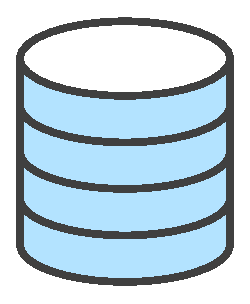
\includegraphics[scale=0.2]{./imagens/forkflow.eps}%
        \end{center}%
        \caption{Workflow de versionamento - passo 01 \label{fig:forkflow01}}%
        \fonte{Atlassian - Comparing Workflows - Acessado em 12/03/2015}%
    \end{figure}%

Passo 2 - Cada integrante da equipe de desenvolvimento cria seu próprio \textit{fork} no github:
    \begin{figure}[htb]%
        \begin{center}
            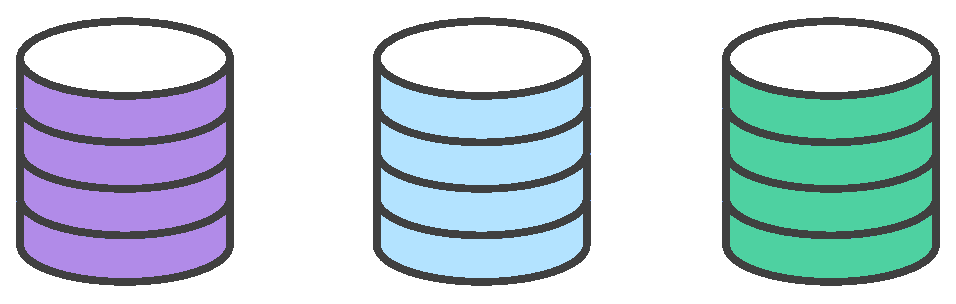
\includegraphics[scale=0.2]{./imagens/forkflow2.eps}%
        \end{center}%
        \caption{Workflow de versionamento - passo 02 \label{fig:forkflow02}}%
        \fonte{Atlassian - Comparing Workflows - Acessado em 12/03/2015}%
    \end{figure}%
    
Passo 3 - Cada integrante da equipe clona seu \textit{fork} em sua máquina local:
    \begin{figure}[htb]%
        \begin{center}
            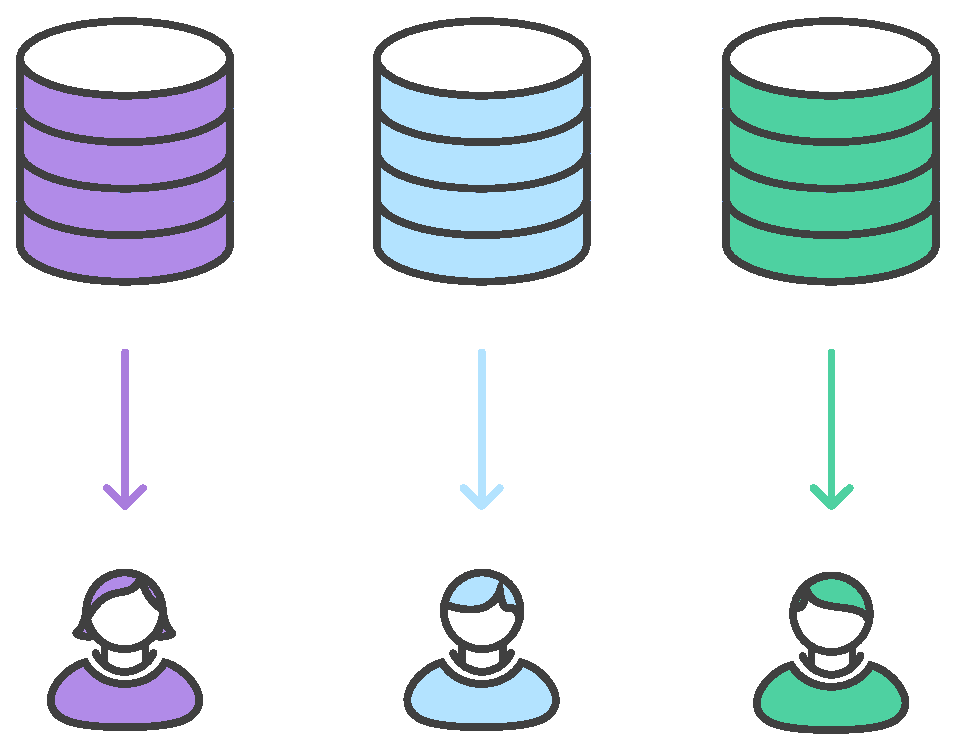
\includegraphics[scale=0.2]{./imagens/forkflow3.eps}%
        \end{center}%
        \caption{Workflow de versionamento - passo 03 \label{fig:forkflow03}}%
        \fonte{Atlassian - Comparing Workflows - Acessado em 12/03/2015}%
    \end{figure}%
\newpage
Passo 4 - Cada integrante da equipe desenvolve suas \textit{features} em \textit{branches} locais:
    \begin{figure}[htb]%
        \begin{center}
            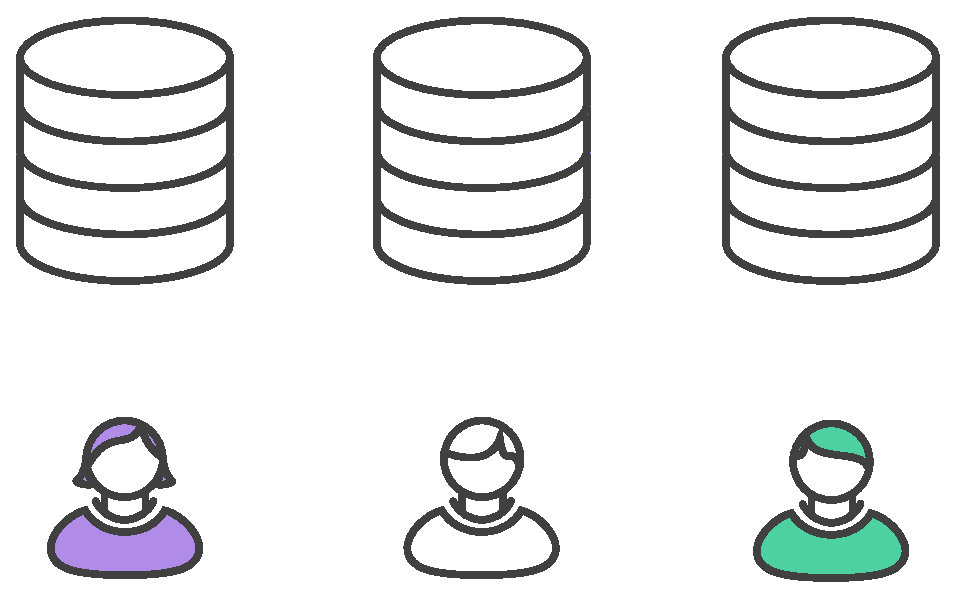
\includegraphics[scale=0.2]{./imagens/forkflow4.eps}%
        \end{center}%
        \caption{Workflow de versionamento - passo 04 \label{fig:forkflow04}}%
        \fonte{Atlassian - Comparing Workflows - Acessado em 12/03/2015}%
    \end{figure}%
    
Passo 5 - Após finalizada a \textit{feature}, o \textit{branch} da \textit{feature} é enviado para o repositório (\textit{fork}) do usuário no github. Caso haja mais de uma pessoa trabalhando na mesma \textit{feature}, recomenda-se que o \textit{branch} da \textit{feature} seja publicado constantemente ao \textit{fork} do usuário de forma que outro desenvolvedor possa utilizar as modificações feitas - realizando um \textit{pull} daquele \textit{branch} para seu repositório.
    \begin{figure}[htb]%
        \begin{center}
            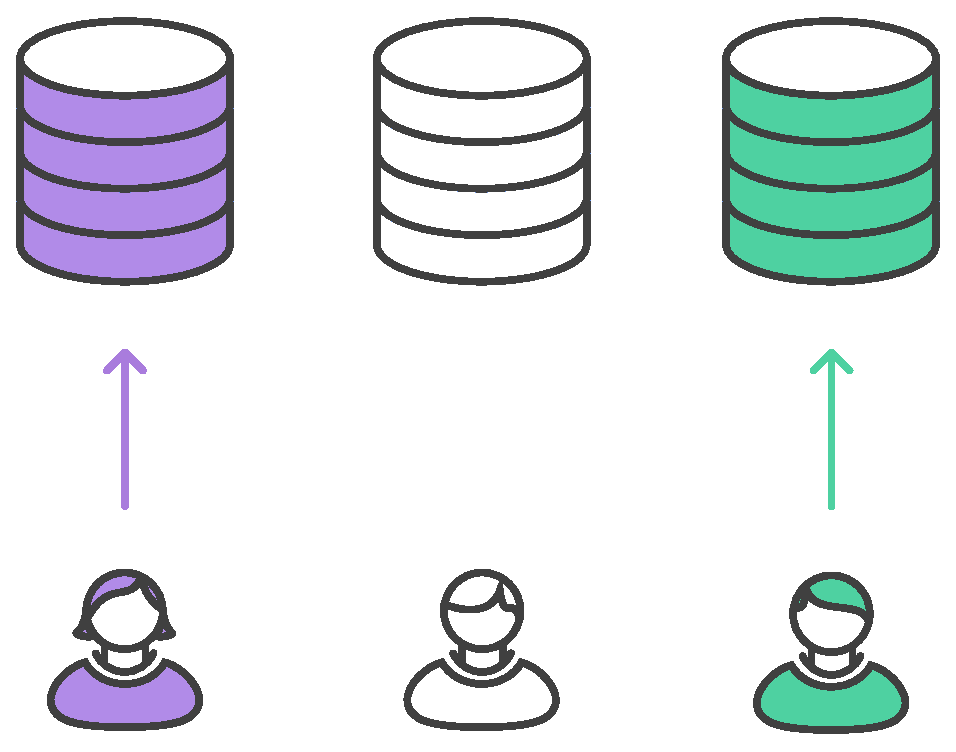
\includegraphics[scale=0.2]{./imagens/forkflow5.eps}%
        \end{center}%
        \caption{Workflow de versionamento - passo 05 \label{fig:forkflow05}}%
        \fonte{Atlassian - Comparing Workflows - Acessado em 12/03/2015}%
    \end{figure}%
\newpage
Passo 6 - Cada responsável por uma \textit{feature} realiza um \textit{Pull-Request} do \textit{branch} de sua \textit{feature} em seu \textit{fork} para o \textit{branch} ``master'' do repositório principal do projeto. Com os \textit{Pull-Requests} o gestor do projeto, no papel de integrador, verifica cada \textit{Pull-Request}, aceita (ou não) o \textit{Pull Request} e integra, uma a uma, as \textit{features} no repositório branch ``master'' de seu repositório local. Neste momento, cada \textit{Pull-Request} representará uma nova \textit{feature} (ou a resolução de algum \textit{bug}/\textit{issue}), e a cada integração deve-se realizar a validação da mesma.
    \begin{figure}[htb]%
        \begin{center}
            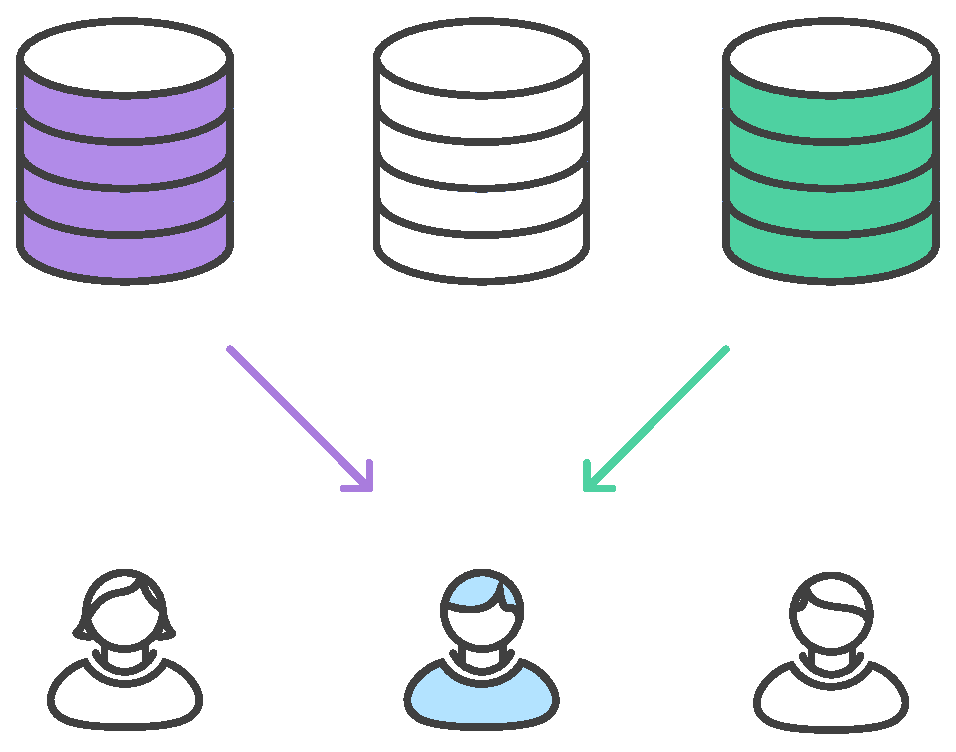
\includegraphics[scale=0.2]{./imagens/forkflow6.eps}%
        \end{center}%
        \caption{Workflow de versionamento - passo 06 \label{fig:forkflow06}}%
        \fonte{Autoria Própria}%
    \end{figure}%

Passo 7 - Após as integrações serem realizadas, o gestor deve enviar o \textit{branch} ``master'' de seu repositório local para o repositório principal do projeto.
    \begin{figure}[htb]%
        \begin{center}
            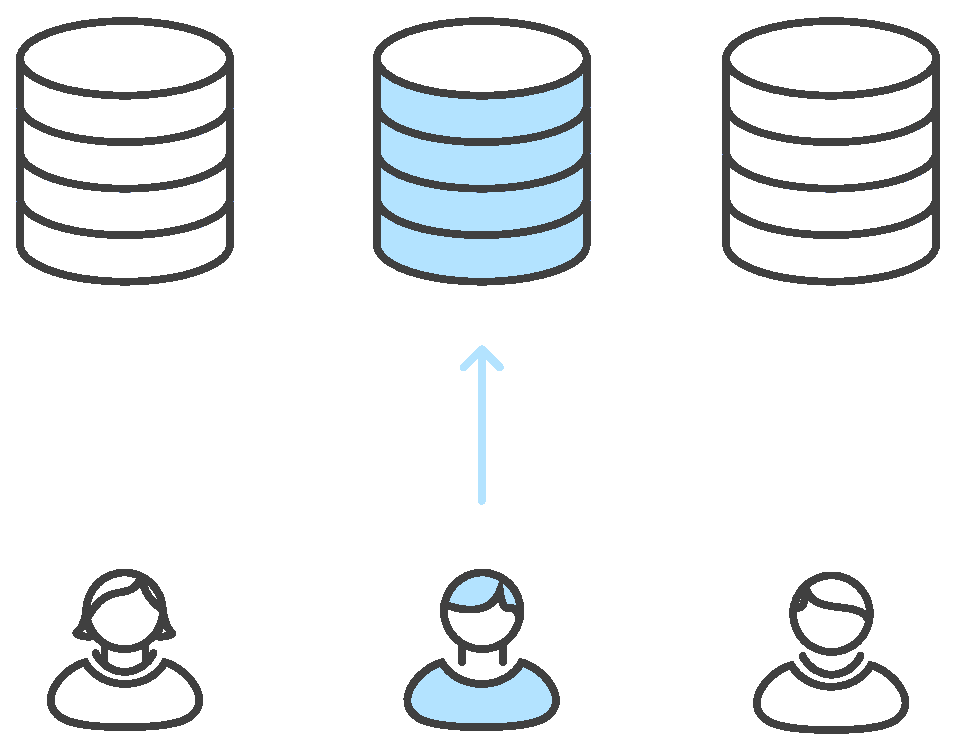
\includegraphics[scale=0.2]{./imagens/forkflow7.eps}%
        \end{center}%
        \caption{Workflow de versionamento - passo 07 \label{fig:forkflow07}}%
        \fonte{Autoria Própria}%
    \end{figure}%
\newpage
Passo 8 - Após a integração das \textit{features} ao repositório principal, todas pessoas que integram a equipe de desenvolvimento sincronizam novamente o \textit{branch} ``master'' de seus \textit{forks} com o \textit{branch} ``master'' do repositório principal.
    \begin{figure}[htb]%
        \begin{center}
            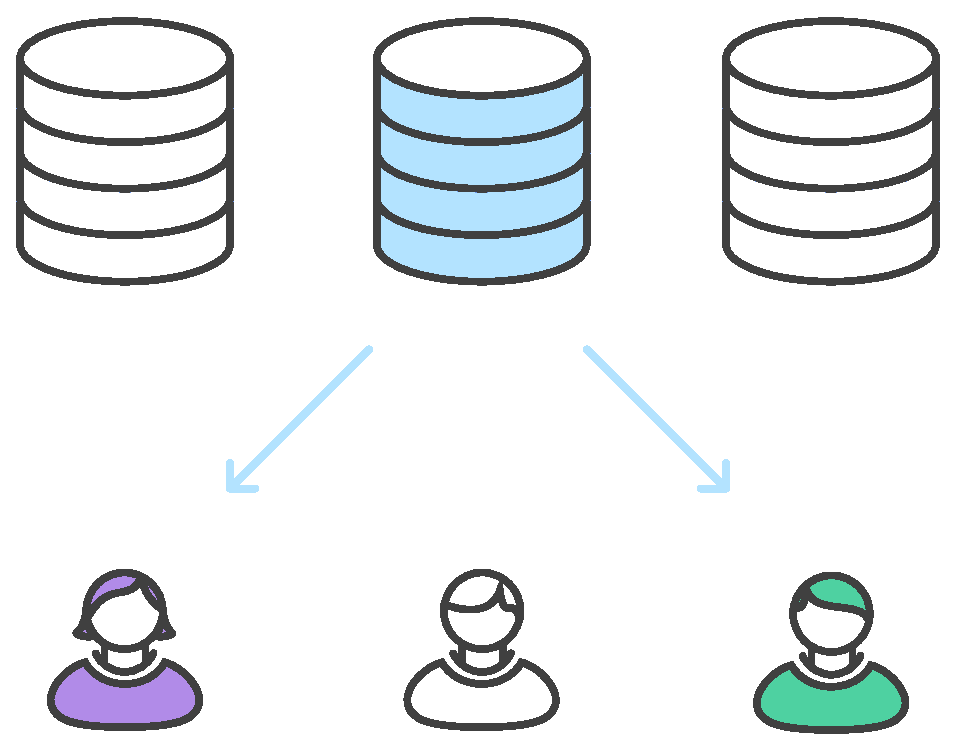
\includegraphics[scale=0.2]{./imagens/forkflow8.eps}%
        \end{center}%
        \caption{Workflow de versionamento - passo 08 \label{fig:forkflow08}}%
        \fonte{Atlassian - Comparing Workflows - Acessado em 12/03/2015}%
    \end{figure}%

Passo 9 - Periodicamente\footnote{A periodicidade depende do modelo de trabalho adotado, que não está definido neste processo de versionamento de código.}, após as integrações realizadas, o gestor define um \textit{release} e marca o repositório com uma \textit{tag} que defina tal \textit{release}, que em seguida será implementado no site em produção\footnote{O processo de implantação de novas versões em produção deve ser definido em outro documento.}.
    \begin{figure}[htb]%
        \begin{center}
            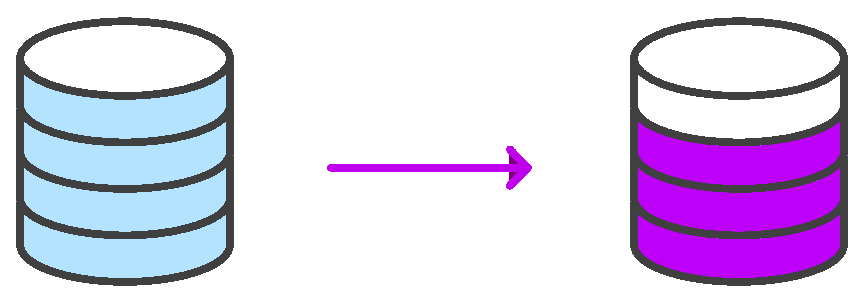
\includegraphics[scale=0.2]{./imagens/forkflow9.eps}%
        \end{center}%
        \caption{Workflow de versionamento - passo 09 \label{fig:forkflow09}}%
        \fonte{Atlassian - Comparing Workflows - Acessado em 12/03/2015}%
    \end{figure}%


% ---
% Conclusão
\chapter{Conclusão}
Para uma tomada de decisão com relação a qual caminho tomar, devem ser analisadas as condições de contorno do projeto visando o desenvolvimento do aplicativo e, posteriormente, sua manutenção e evolução. 

Neste sentido, é fundamental levar em conta que a \gls{sal} não possui uma equipe de desenvolvimento fixa e tem trabalhado com o modelo de Consultores temporários, o que impõe duas grandes consequências, sendo elas a equipe de tamanho reduzido e a alta rotatividade dos profissionais.

Outro ponto a ser considerado é a limitação econômica do projeto, e a decisão político-estratégica de priorizar a utilização de softwares e tecnologias livres e abertas.

Dessa forma, a aparentem melhor decisão seria escolher pelo modelo de desenvolvimento híbrido, utilizando o framework Cordova para empacotamento de APPs. Tal opção além de reduzir a necessidade de maior diversidade técnica na equipe também reduz a quantidade de trabalho para o desenvolvimento de aplicativo para diversas plataformas. Outra vantagem é que os desenvolvedores que atuam na plataforma web também podem contribuir com o desenvolvimento do APP, aproveitando melhor os poucos recursos destinados ao projeto.

Com relação ao framework de \gls{ui} que será utilizado, a decisão deve ser tomada com base numa experimentação inicial por parte da equipe que iniciará o desenvolvimento do aplicativo, para que a adaptação da equipe de desenvolvimento ao framework seja a mais rápida possível.


% ---

% ----------------------------------------------------------
% ELEMENTOS PÓS-TEXTUAIS
% ----------------------------------------------------------
\postextual

% ----------------------------------------------------------
% Referências bibliográficas
% ----------------------------------------------------------
\bibliography{produto}

% ---
% inserir lista de abreviaturas e siglas


% ----------------------------------------------------------
% Glossário
% ----------------------------------------------------------
%
% Consulte o manual da classe abntex2 para orientações sobre o glossário.
%
%\glossary

% ----------------------------------------------------------
% Apêndices
% ----------------------------------------------------------

% ---
% Inicia os apêndices
% ---
%\begin{apendicesenv}

% Imprime uma página indicando o início dos apêndices
%\partapendices

% ----------------------------------------------------------
%\chapter{Primeiro apêndice}
% ----------------------------------------------------------

%\end{apendicesenv}
% ---

% ----------------------------------------------------------
% Anexos
% ----------------------------------------------------------

% ---
% Inicia os anexos
% ---
%\begin{anexosenv}

% Imprime uma página indicando o início dos anexos
%\partanexos

% ---
%\chapter{Primeiro Anexo}

%\end{anexosenv}

%---------------------------------------------------------------------
% INDICE REMISSIVO
%---------------------------------------------------------------------
%
%\phantompart
%
%\printindex
% Define nome e preâmbulo do glossário
\phantompart
\renewcommand{\glossaryname}{Gloss\'{a}rio}
%\renewcommand{\glossarypreamble}{Esta é a descrição do glossário. Experimente}
% ---
% Traduções para o ambiente glossaries
\providetranslation{Glossary}{Glossário}
\providetranslation{Acronyms}{Siglas}
\providetranslation{Notation (glossaries)}{Notação}
\providetranslation{Description (glossaries)}{Descrição}
\providetranslation{Symbol (glossaries)}{Símbolo}
\providetranslation{Page List (glossaries)}{Lista de Páginas}
\providetranslation{Symbols (glossaries)}{Símbolos}
\providetranslation{Numbers (glossaries)}{Números}
% ---
% Estilo de glossário
\setglossarystyle{altlist}
\setacronymstyle{long-short-desc}
% ---
% Imprime o glossário
%\cleardoublepage
\phantomsection
\printindex[sort=word]

%---------------------------------------------------------------------
% Formulário de Identificação (opcional)
%---------------------------------------------------------------------
%\chapter*[Formulário de Identificação]{Formulário de Identificação}
%\addcontentsline{toc}{chapter}{Exemplo de Formulário de Identificação}
%\label{formulado-identificacao}
%
%%Exemplo de Formulário de Identificação, compatível com o Anexo A (informativo) da ABNT NBR 10719:2011. Este formulário não é um anexo. Conforme definido na norma, ele é o último elemento pós-textual e opcional do relatório.
%
%\bigskip
%
%\begin{tabular}{|p{9cm}|p{5cm}|}
%\hline
%\multicolumn{2}{|c|}{\textbf{\large Dados do Relatório Técnico}}\\
%\hline
%\multirow{4}{9cm}{{Relatório contendo avaliação e propostas de melhorias técnicas para ferramentas e aplicações de consulta pública, incluindo plugins}}& Classificação de segurança\\
%                    & \\
%                   \cline{2-2}
%                   & No.\\
%                    & 1 \\
%				
%\hline
%Relatório Técnico & 13/03/2015\\
%\hline
%{Projeto Democratização de Informações no Processo de Elaboração Normativa} & No. BRA/07/004\\
%\hline
%\multicolumn{2}{|l|}{Diego Rabatone Oliveira} \\
%\hline
%\multicolumn{2}{|l|}{Secretaria de Assuntos Legislativos do Ministério da Justiça (SAL/MJ)} \\
%\hline
%\multicolumn{2}{|l|}{Programa das Nações Unidas para o Desenvolvimento (PNUD)} \\
%\hline
%\multicolumn{2}{|l|}{\multirow{1}{0.9\textwidth}{Este produto objetiva realizar uma avaliação técnica das ferramentas e aplicações de consulta pública do projeto “Pensando o Direito”, do Ministério da Justiça. Além da avaliação serão também propostas melhorias dos recursos já existentes, tendo como objetivo secundário a publicização de tais melhorias enquanto ferramentas livres que possam ser reutilizadas pela sociedade. Para o desenvolvimento deste trabalho foi utilizada metodologia de desenvolvimento ágil, com definição de tarefas a serem realizada e sprints para a realização das mesmas. Resulta ainda deste trabalho uma recomendação de método de trabalho da equipe de desenvolvimento.}}\\[5cm]
%\hline
%\multicolumn{2}{|l|}{\multirow{1}{0.9\textwidth}{Palavras-Chaves: Wordpress, \mc, \pdp, Métodos Ágeis}}\\[0.7cm]
%\hline
%\multicolumn{2}{|l|}{
%1$^a$Edição \hfill \pageref{LastPage} páginas \hfill Volume 1 \hfill Nº de classificação \phantom{XXXX}} \\
%\hline
%\multicolumn{2}{|l|}{ISSN \phantom{XXXX}\hfill Tiragem \phantom{XXXX}} \\
%\hline
%%\multicolumn{2}{|l|}{Distribuidor} \\
%%\hline
%%\multicolumn{2}{|l|}{Observações/notas}\\[3cm]
%%\hline
%\end{tabular}
%
\end{document}
